% LaTeX Template for short student reports.
% Source of the template: https://gist.github.com/cpmpercussion/a6fb23976f3a8bf5c045f54ab62ee057
% Citations should be in bibtex format and go in references.bib
\documentclass[a4paper, 11pt]{article}
\usepackage[top=3cm, bottom=3cm, left = 2cm, right = 2cm]{geometry} 
\geometry{a4paper} 
\usepackage[utf8]{inputenc}
\usepackage{textcomp}
\usepackage{graphicx} 
\usepackage{amsmath,amssymb}  
\usepackage{bm}  
\usepackage{listings}
\usepackage{mdframed}
\usepackage{tablefootnote}
\usepackage[bottom]{footmisc}
\usepackage[pdftex,bookmarks,colorlinks=false,breaklinks]{hyperref}  
%\hypersetup{linkcolor=black,citecolor=black,filecolor=black,urlcolor=black} % black links, for printed output
\usepackage{memhfixc} 
\usepackage{pdfsync}  
\usepackage{fancyhdr}
\pagestyle{fancy}

\title{CVPR 2023 Project Report - CNN Classifier}
\author{Michele Scomina}
\setlength{\headheight}{14pt}
%\date{}

\begin{document}
% No indentation
\setlength{\parindent}{0pt}
% Paragraph spacing
\setlength{\parskip}{3pt}
\maketitle
\tableofcontents
\definecolor{codegreen}{rgb}{0,0.6,0}
\definecolor{codegray}{rgb}{0.5,0.5,0.5}
\definecolor{codepurple}{rgb}{0.58,0,0.82}
\definecolor{backcolour}{rgb}{0.95,0.95,0.92}
\lstdefinestyle{mystyle}{
    backgroundcolor=\color{backcolour},   
    commentstyle=\color{codegreen},
    keywordstyle=\color{magenta},
    numberstyle=\tiny\color{codegray},
    stringstyle=\color{codepurple},
    basicstyle=\ttfamily\footnotesize,
    breakatwhitespace=false,         
    breaklines=true,                 
    captionpos=b,                    
    keepspaces=true,                 
    numbers=left,                    
    numbersep=5pt,                  
    showspaces=false,                
    showstringspaces=false,
    showtabs=false,                  
    tabsize=2
}

\pagebreak

\section{Problem Statement}
The project requires the implementation of an image classifier based on convolutional neural networks.
The provided dataset (from \cite{lazebnik2006beyond}) contains 15 categories (office, kitchen, living room,
bedroom, store, industrial, tall building, inside city, street, highway, coast, open country, mountain,
forest, suburb), and is already divided in training set and test set.\footnote{Of 1500 and 3000 images respectively.} An example of each category is
shown in Fig. \ref{fig:dataset_preview}.

\begin{figure}[h]
    \centering
    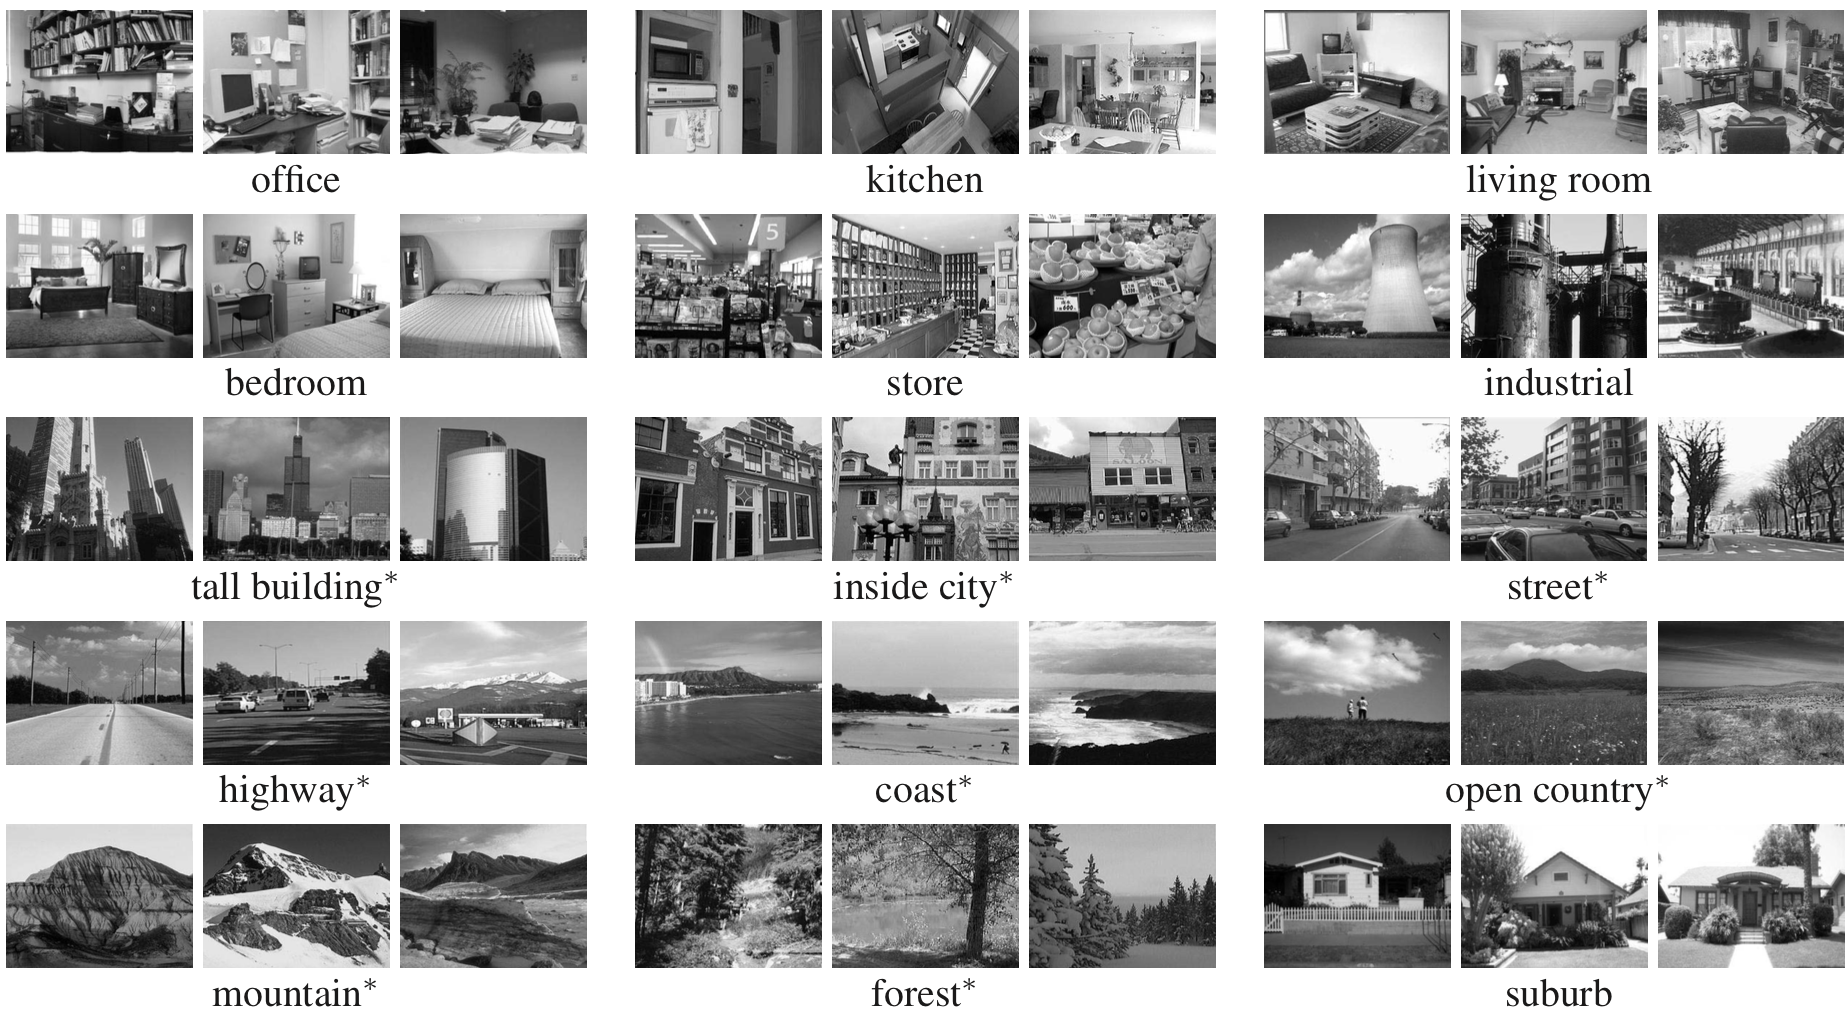
\includegraphics[width=1.0\textwidth]{dataset_preview.png}
    \caption{Examples of images from each of the 15 categories of the provided dataset (the same as \cite{lazebnik2006beyond}).}
    \label{fig:dataset_preview}
\end{figure}

\vspace{10pt}

The tasks of the given project can be divided in three parts:
\begin{enumerate}
    \item \textbf{Base reference model}: Initialization and training of a CNN model with a fixed architecture, without applying any data augmentation.
    \item \textbf{Optimized model}: Optimization of the previous result by making use of data augmentation techniques and different architectures.
    \item \textbf{Transfer learning}: Improvement on the previous results through transfer learning, by fine-tuning a pre-trained model to the given dataset and by using the pre-trained model as a feature extractor for a SVM classifier.
\end{enumerate}

\pagebreak

% Dataset table with labels
\begin{table}[b]
    \centering
    \begin{tabular}{|c|l|c|l|c|l|}
    \hline
    Label & Description & Label & Description & Label & Description \\
    \hline
    0 & Bedroom & 5 & Inside city & 10 & Open country \\
    1 & Coast & 6 & Kitchen & 11 & Store \\
    2 & Forest & 7 & Living room & 12 & Street \\
    3 & Highway & 8 & Mountain & 13 & Suburb \\
    4 & Industrial & 9 & Office & 14 & Tall building \\
    \hline
    \end{tabular}
    \caption{Dataset labels.}
    \label{tab:labels}
\end{table}

\section{Tools, libraries and structure}
The project has been developed in Python, using the following libraries:
\begin{itemize}
    \item \textbf{PyTorch} for the implementation of the CNN models.
    \item \textbf{Scikit-learn} for the implementation of the SVM classifier.
    \item \textbf{Matplotlib} for the visualization of the results.
    \item \textbf{Seaborn} for the visualization of the confusion matrix.
    \item \textbf{Scipy} for the estimates of the confidence intervals. 
\end{itemize}

The project has also been designed to be as modular as possible, in order to allow easy testing
of different architectures and hyperparameters. There might then be some differences with the displayed 
code.\footnote{More specifically, some of the variables in this report have been replaced with constants for the specific task, for ease of readability.}\\
The main folders of the project are:
\begin{itemize}
    \item \textbf{dataset/}: contains the dataset, respectively in /train/ and /test/.
    \item \textbf{models/}: contains the code for the implementation of the CNN models, as well as the saved models.
    \item \textbf{plots/}: contains the visualization of the results through graphs and confusion matrices.
    \item \textbf{tasks/}: contains the code for the implementation of the tasks.
    \item \textbf{utils/}: contains various helper libraries, like the training and plot code.
\end{itemize}
The project can be run through the \textbf{main.py} file, which will train the models and
save the various losses and accuracies graphs during training in the \textbf{plots/} folder,
as well as save the trained models in the \textbf{models/} folder and the test accuracies in \textbf{results.txt}.\\
All of the code is available on GitHub at \url{https://github.com/MScomina/computer-vision-project}.

\pagebreak

\section{Base reference model}

The first task of the project consists in training a CNN model with the following architecture:
\begin{table}[h]
    \centering
    \begin{tabular}{l|l|l}
        \textbf{\#} & \textbf{type} & \textbf{size} \\
        \hline
        1 & Image Input & 64x64x1 \\
        2 & Convolution & 8 3x3 convolutions with stride 1 \\
        3 & ReLU & \\
        4 & Max Pooling & 2x2 max pooling with stride 2 \\
        5 & Convolution & 16 3x3 convolutions with stride 1 \\
        6 & ReLU & \\
        7 & Max Pooling & 2x2 max pooling with stride 2 \\
        8 & Convolution & 32 3x3 convolutions with stride 1 \\
        9 & ReLU & \\
        10 & Fully Connected & 15 \\
        11 & Softmax & softmax \\
        12 & Classification Output & crossentropyex \\
    \end{tabular}
    \caption{Layout of the base reference model.}
    \label{tab:base_model}
\end{table}
\\
The model has to be initialized with starting weight values sampled from a normal distribution with mean 0
and standard deviation 0.01 and no bias. The model has to then be trained on minibatches of size 32 on a 
85/15 train/validation split.

\subsection{Implementation of the model}
\lstset{style=mystyle}
This architecture can be implemented in PyTorch by creating a torch.nn.Module class with the following layers:
\begin{lstlisting}[language=Python]
import torch.nn as nn
self.layers = nn.Sequential(
    nn.Conv2d(in_channels=1, out_channels=8, kernel_size=3, stride=1, padding=1),
    nn.ReLU(),
    nn.MaxPool2d(kernel_size=2, stride=2),
    nn.Conv2d(in_channels=8, out_channels=16, kernel_size=3, stride=1, padding=1),
    nn.ReLU(),
    nn.MaxPool2d(kernel_size=2, stride=2),
    nn.Conv2d(in_channels=16, out_channels=32, kernel_size=3, stride=1, padding=1),
    nn.ReLU(),
    nn.Flatten(),
    nn.Linear(in_features=8192, out_features=15)
)
\end{lstlisting}
The number of final features can be calculated from the following formula, considering that every 2x2 
max pooling layer with stride 2 halves the channels' sizes:
\begin{equation*}
    \text{in\_features} = \left(\frac{\text{image\_size}}{4}\right)^2 \cdot \text{n\_of\_final\_kernels} = \left(\frac{64}{4}\right)^2 \cdot 32 = 8192
\end{equation*}
The Convolutional and Linear layers are then initialized with the following code:
\begin{lstlisting}[language=Python]
if type(m) == nn.Conv2d or type(m) == nn.Linear:
    nn.init.normal_(m.weight, mean=0.0, std=0.01)
    if m.bias is not None:
        nn.init.constant_(m.bias, 0.0)
\end{lstlisting}

\pagebreak

\subsection{Training of the model}

\subsubsection{Dataset loading}
First, the transformations to be applied to the images are defined:
\begin{lstlisting}[language=Python]
from torchvision import transforms, datasets
transform = transforms.Compose([
    transforms.Resize((64, 64)),
    transforms.Grayscale(),
    transforms.ToTensor(),
    transforms.Lambda(lambda x: x * 255)
])
\end{lstlisting}
This transformation rescales the images anisotropically to a size of 64x64, converts them to 
grayscale\footnote{since ImageFolder loads them as RGB images, therefore with 3 channels}, converts them to a tensor and then
scales the values back to [0,255]\footnote{since ToTensor converts the image to a tensor with values in the range [0,1]}.\\

The dataset is then loaded into three DataLoaders (train, validation and test) 
by employing ImageFolder, using the previously defined transformations: 
\begin{lstlisting}[language=Python]
from torch.utils.data import DataLoader
from datasets import ImageFolder

full_training_data = ImageFolder(root="dataset/train", transform=transform)
test_dataset = ImageFolder(root="dataset/test", transform=transform)

train_size = int(0.85 * len(full_training_data))
val_size = len(full_training_data) - train_size
train_dataset, val_dataset = torch.utils.data.random_split(full_training_data, [train_size, val_size])

train_loader = DataLoader(train_dataset, batch_size=batch_size, shuffle=True)
val_loader = DataLoader(val_dataset, batch_size=batch_size, shuffle=True)
test_loader = DataLoader(test_dataset, batch_size=batch_size, shuffle=True)
\end{lstlisting}

\subsubsection{Training}
For the choice of hyperparameters, the following values have been used:
\begin{itemize}
    \item \textbf{Learning rate}: 0.001. This value has been chosen because it is commonly used in CNNs (because it's not too big to overshoot nor too small to slow down the training too much).
    \item \textbf{Momentum}: 0.9. This value helps the model converge faster and avoid getting stuck in local minima.
    \item \textbf{Patience}: 10. This value describes the number of epochs without improvement after which the training is stopped. 
    10 epochs were chosen as a reasonable period for the model to converge.
\end{itemize}
After initializing the model, the optimizer (stochastic gradient descent) and the loss function (cross entropy) are defined:
\begin{lstlisting}[language=Python]
model = CNN_task_1()
optimizer = torch.optim.SGD(model.parameters(), lr=0.001, momentum=0.9)
loss_function = nn.CrossEntropyLoss()
\end{lstlisting}

\pagebreak

The model is then trained using the following code:
\begin{lstlisting}[language=Python]
model.train()
for x, y in iter(train_loader):
    optimizer.zero_grad()
    y_pred = model(x)
    l = loss_function(y_pred, y)
    l.backward()
    optimizer.step()
\end{lstlisting}

The training and validation losses and accuracies are calculated at each epoch, and the validation loss 
is used as a stopping criterion (if it doesn't improve for 10 epochs, the training is stopped):

\begin{lstlisting}[language=Python]
model.eval()
loss = 0
correct = 0
total = 0
with torch.no_grad():
    for x, y in iter(loader):
        y_pred = model(x)
        l = loss_function(y_pred, y)
        loss += l.item()
        _, predicted = torch.max(y_pred.data, 1)
        total += y.size(0)
        correct += (predicted == y).sum().item()
loss /= len(loader)
accuracy = correct / total
\end{lstlisting}

\subsubsection{Results}
The model was trained for a maximum of 300 epochs. 
The training and validation losses and accuracies are as follows:
\begin{figure}[h]
    \centering
    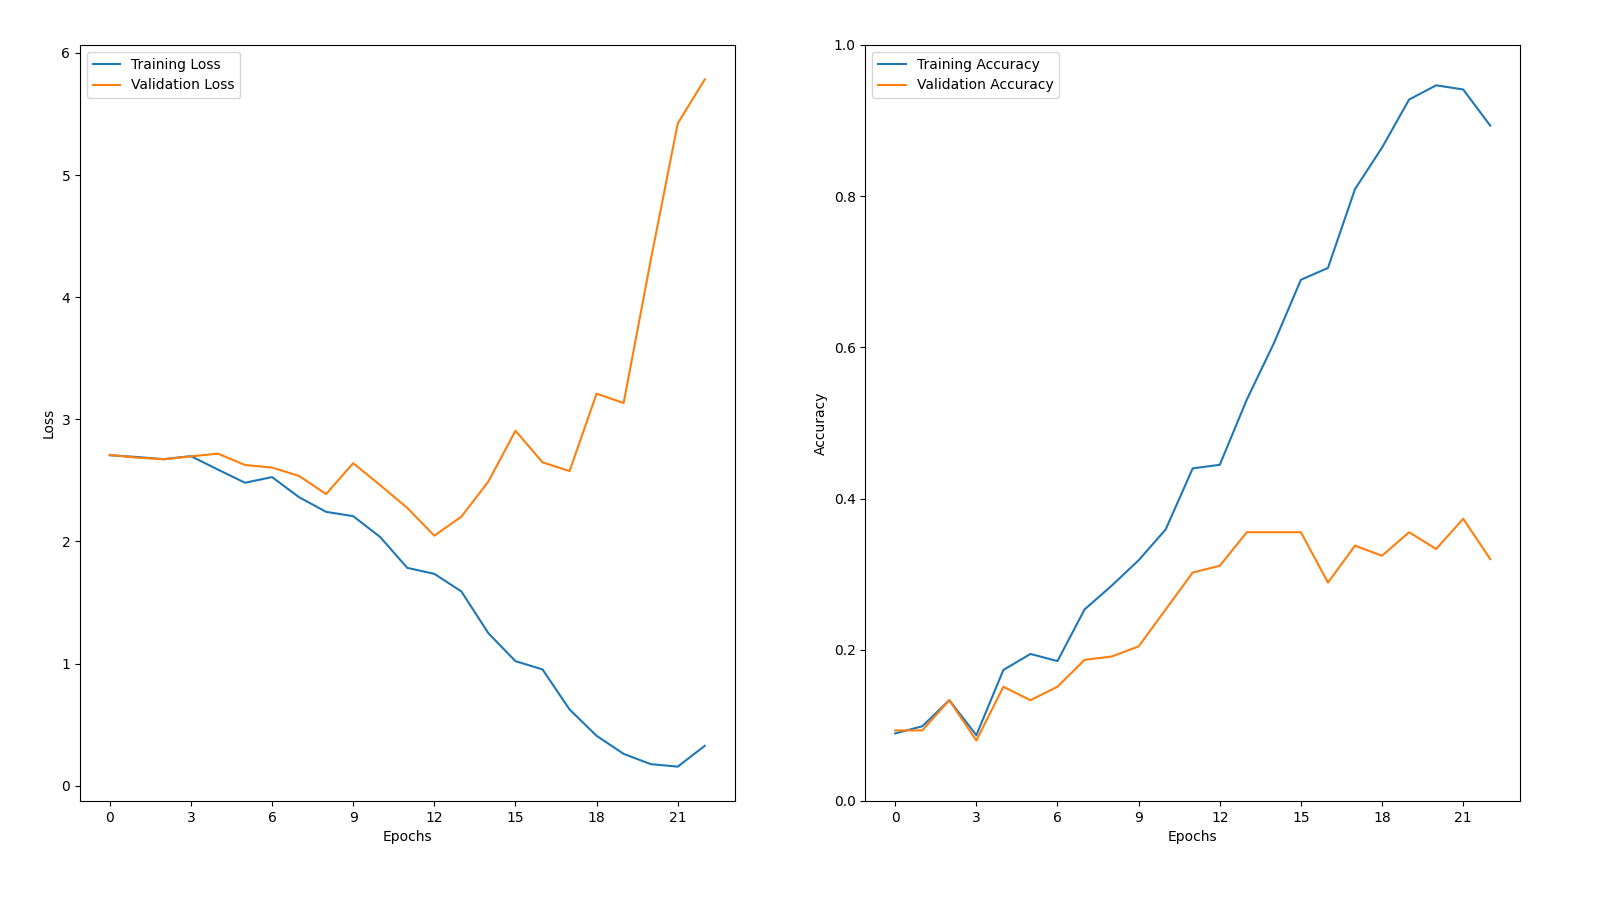
\includegraphics[width=0.75\textwidth]{loss_and_accuracy_task_1.png}
    \caption{Training and validation losses and accuracies of the base reference model.}
    \label{fig:task1_loss_accuracy}
\end{figure}

As expected, without using any data augmentation techniques or batch normalization, the model quickly starts overfitting just after a few epochs.

\pagebreak

The confusion matrix of the model on the test set is as follows:
\begin{figure}[h]
    \centering
    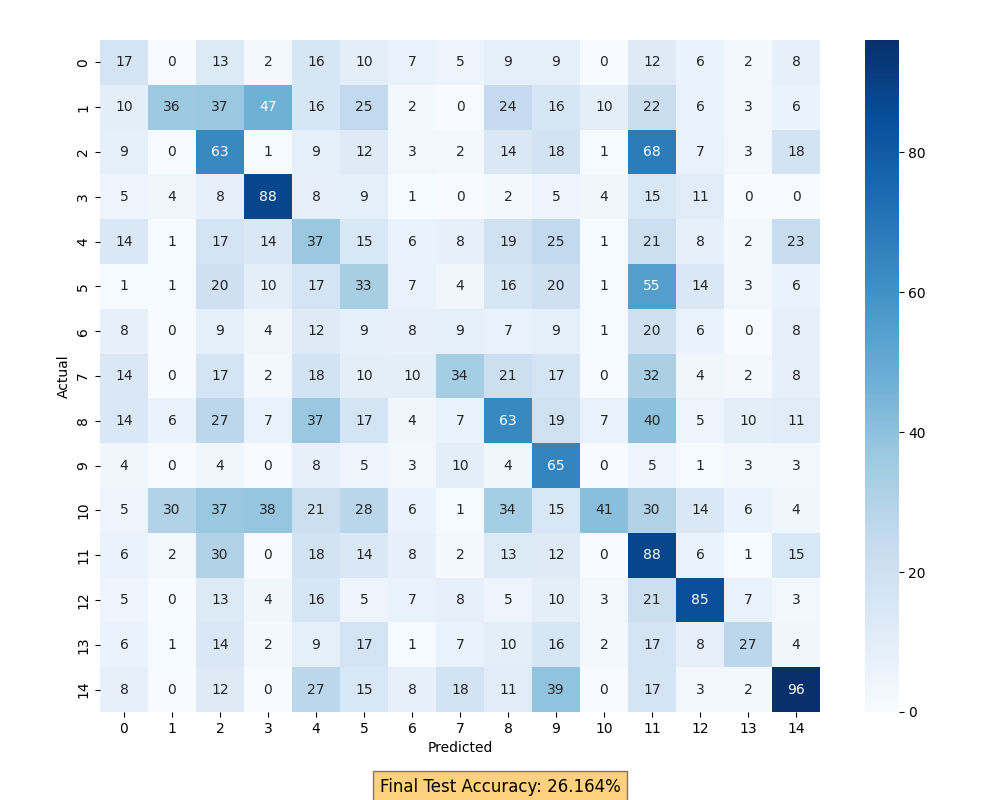
\includegraphics[width=0.66\textwidth]{confusion_matrix_task_1.png}
    \caption{Confusion matrix of the base reference model on the test set.}
    \label{fig:task1_confusion_matrix}
\end{figure}

The average test accuracy of the model is 27.9±1.9\%\footnote{95\% confidence interval over 10 runs using the t-distribution.}\\
From the confusion matrix, it's clear that the model primarily specialized in the easiest categories,
like \textit{tall buildings} (label 14)[\ref{tab:labels}]. It's likely that the model wasn't able to learn
the more complex categories because of the lack of data augmentation techniques and batch normalization, 
and therefore the model just fitted the training set without generalizing well to the test set.\\
Nonetheless, the model performed better than a random classifier, which would have an expected accuracy of approximately 7\%.

\section{Optimized model}
The second task of the project consists in improving the previous result by applying data augmentation
techniques and using different architectures. The following techniques have been used:

\begin{itemize}
    \item \textbf{Data augmentation}: Data augmentation can be applied to the training set in order to improve the generalization of the model by effectively providing more data for training.
    \item \textbf{Regularization}: Regularization techniques can be applied to the model in order to prevent overfitting and further improve the generalization of the model.
    \item \textbf{Architectural changes}: The architecture of the model can be changed in order to improve the performance.
\end{itemize}

\subsection{Data augmentation}
One of the main issues of the previous model is that it overfits the training set very quickly.
This is due to the fact that the dataset is relatively small (only 1500 images for 15 categories).
In order to improve the generalization of the model, data augmentation techniques can be applied to the training set.
The following data augmentation techniques have been applied:
\begin{itemize}
    \item \textbf{Random horizontal flip}: The image is flipped horizontally with a probability of 0.5.
    \item \textbf{Random rotation}: The image is rotated by a random angle between -20 and 20 degrees.
    \item \textbf{Random crop}: The image is randomly cropped first into a 160x160 image, and then resized to 64x64 with a probability of 0.33.
    \item \textbf{Random noise}: The image is perturbed with Gaussian noise with mean 0 and a standard deviation 0.02.
    \item \textbf{Data normalization}: The image is normalized with mean 0.5 and standard deviation 0.5.
\end{itemize}
These data augmentation techniques can be easily added to the dataset by modifying the transformations of the training set specifically:
\begin{lstlisting}[language=Python]
data_augmentation_transform = transforms.Compose([
    transforms.RandomHorizontalFlip(p=0.5)
    transforms.RandomRotation(degrees=20),
    transforms.RandomChoice([
        transforms.Resize((64, 64)),
        transforms.Resize((64, 64)),
        transforms.Compose([
            transforms.RandomCrop(160),
            transforms.Resize(64)
        ])
    ]),
    transforms.Grayscale(),
    transforms.ToTensor(),
    transforms.Lambda(lambda x: torch.clamp(x + 0.02*torch.randn_like(x),min=0.,max=1.)),
    transforms.Normalize(mean=[0.5], std=[0.5])
])
\end{lstlisting}

These data augmentation techniques enhance the performance of the model by improving its generalization.
Data augmentation does present some drawbacks, though:
\begin{itemize}
    \item The model requires more training time and a higher patience value of 30, since it takes longer to train and converge on the augmented data.
    \item The learning rate has to be lowered to 0.0003, since the model starts to experience the "dying ReLU" problem.\footnote{The "dying ReLU" problem is a phenomenon that occurs when a lot of the neurons of the model always output 0, due to the ReLU function being 0 for negative values, slowing down the training of the model.}
\end{itemize}
The average test accuracy of the model with data augmentation is 43.7±2.5\%, which is a significant improvement over the previous model.
The model also stops overfitting on the training set.
\pagebreak

\subsection{Regularization}
Another way to improve the generalization of the model is to apply regularization techniques.
The following regularization techniques have been applied:
\begin{itemize}
    \item \textbf{Batch normalization}: Batch normalization is a technique that normalizes the output of the previous layer by subtracting the batch mean and dividing by the batch standard deviation. 
    This technique helps the model to converge faster and to not get stuck in local minima. \cite{ioffe2015batch}
    \item \textbf{Dropout}: Dropout is a technique that randomly sets a fraction of the input units of a layer to 0 during training.
    The dropout rate has been set to 0.2 due to the model not overfitting with data augmentation, therefore not requiring a high dropout rate.
\end{itemize}
These regularization techniques can be easily added to the model by changing the layers of the model:
\begin{lstlisting}[language=Python]
nn.Conv2d(in_channels=n, out_channels=m, kernel_size=3, stride=1, padding=1),
nn.BatchNorm2d(m),
nn.ReLU(),
nn.Dropout(p=0.2),
nn.MaxPool2d(kernel_size=2, stride=2),
\end{lstlisting}
The final average test accuracy of the model with data augmentation and regularization is 54.2±1.9\%.
The model also converges much faster than using only data augmentation.

\subsection{Architectural changes}
The final way to improve the performance of the model is to change its architecture.
The following architectural changes have been applied:
\begin{itemize}
    \item \textbf{Swish activation}: Implementation of the Swish function, which is defined as follows:
    \begin{equation*}
        \text{Swish}(x) = x \cdot \sigma (\beta x)
    \end{equation*}
    where $\sigma(x)$ is the sigmoid function and $\beta$ is a hyperparameter. This function effectively solves the "dying ReLU" problem due to its non-zero gradient for negative values. \cite{ramachandran2017searching}\\
    For this specific model, $\beta = 0.8$ has been chosen.
    \item \textbf{Bigger kernel sizes}: Use of a 7x7 kernel size in the first convolutional layer and 5x5 on the second one.
    \item \textbf{More layers}: The addition of another 3x3 convolutional layer with 64 output channels and another max pooling layer allows more complex patterns to be learned.
    \item \textbf{Kaiming initialization}: Use of the Kaiming initialization \cite{he2015delving} instead of the normal initialization. 
    Although the Kaiming initialization has been designed for ReLU, it works well with Swish too due to its similar shape.\footnote{In fact, $\beta \rightarrow \infty \implies \text{Swish}(x) \rightarrow \text{ReLU}(x)$.}
    \item \textbf{Ensemble of models}: Use of an ensemble of 10 models, each trained on the dataset indipendently of each other.
    The final prediction is the average of the predictions of the 10 models. \cite{szegedy2015going}
\end{itemize}

\pagebreak

The Swish function has to be manually implemented in PyTorch as follows, and then used as an activation function in place of ReLU:
\begin{lstlisting}[language=Python]
class Swish(nn.Module):
    def __init__(self, beta=1.0):
        super().__init__()
        self.beta = beta
    def forward(self, x):
        return x * torch.sigmoid(self.beta * x)
\end{lstlisting}
The Kaiming initialization can be applied to the model by changing the initialization of the layers as follows:
\begin{lstlisting}[language=Python]
def _init_weights(self, m):
    if type(m) == nn.Conv2d or type(m) == nn.Linear:
        if type(m) == nn.Conv2d:
            nn.init.kaiming_normal_(m.weight, mode="fan_out", nonlinearity="relu")
        else:
            nn.init.kaiming_normal_(m.weight, mode="fan_in", nonlinearity="relu")
\end{lstlisting}
The model's training and validation losses and accuracies are as follows:
\begin{figure}[h]
    \centering
    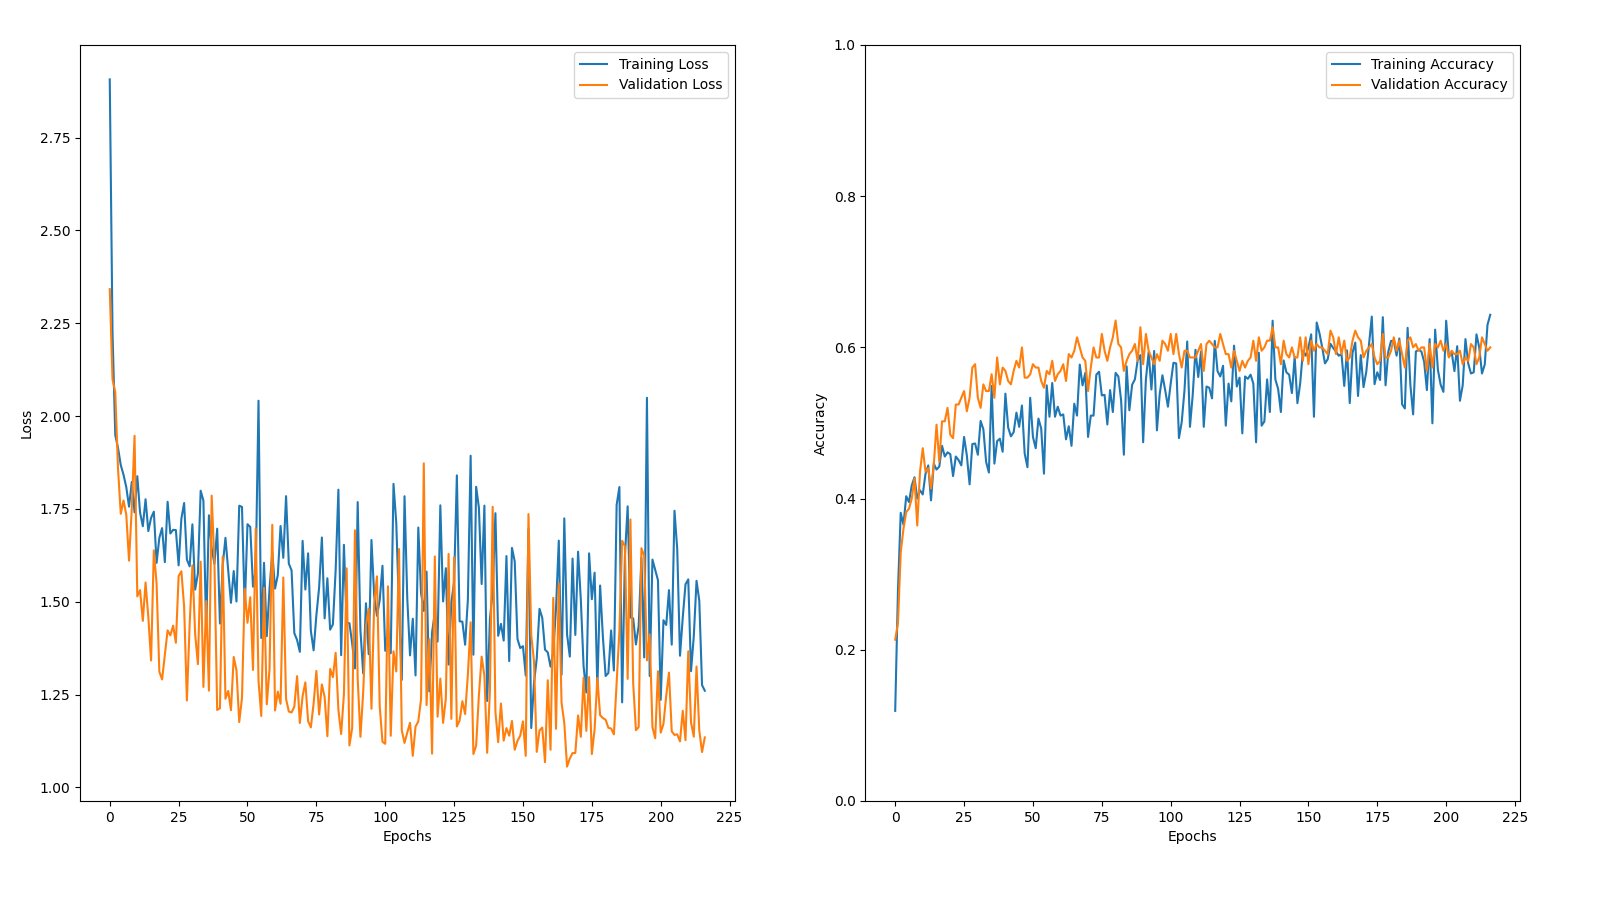
\includegraphics[width=0.75\textwidth]{loss_and_accuracy_task_2.png}
    \caption{Training and validation losses and accuracies of the optimized model.}
    \label{fig:task2_loss_accuracy}
\end{figure}

As shown, the model performs much better and doesn't overfit the training data.

\pagebreak

The confusion matrix of the model on the test set is as follows:
\begin{figure}[h]
    \centering
    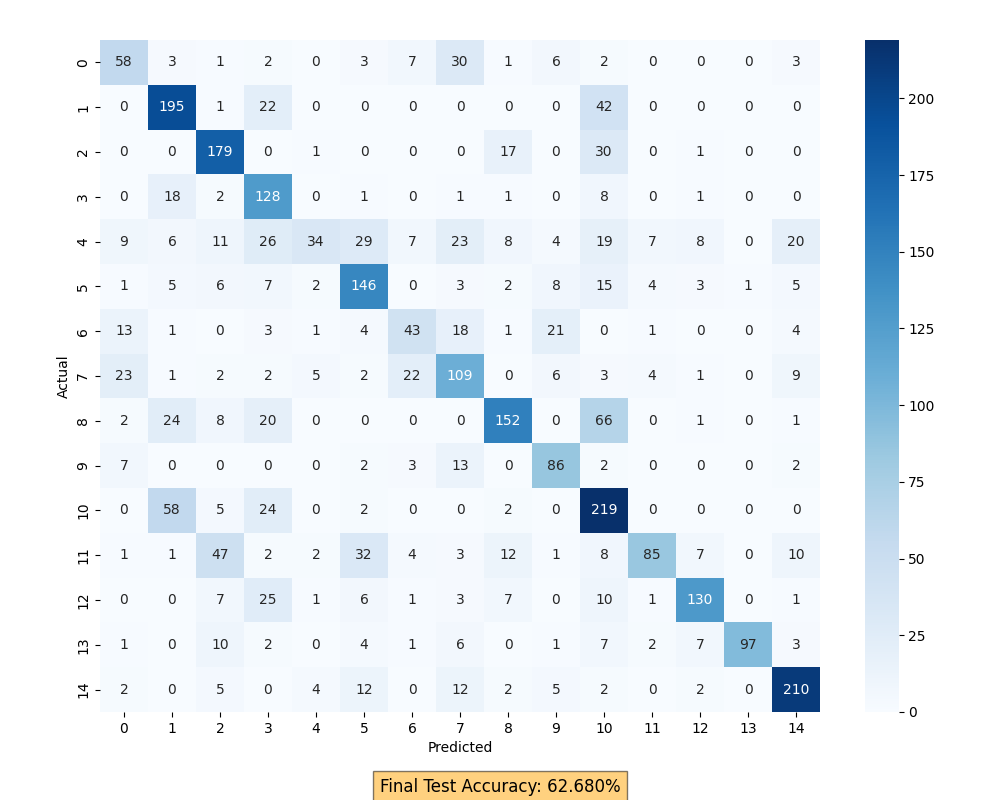
\includegraphics[width=0.66\textwidth]{confusion_matrix_task_2.png}
    \caption{Confusion matrix of the optimized model on the test set.}
    \label{fig:task2_confusion_matrix}
\end{figure}

By increasing the patience to 50, the final test accuracy of the ensemble of models ends up being 62.7\%, 
which is a significant improvement over the previous model.\footnote{Due to the model's complexity and the associated computational limitations, the model was only trained once.}

\section{Transfer learning}
The third task consists in using a previously trained model and fine-tuning it to the given dataset.

The chosen model is the AlexNet model \cite{krizhevsky2012imagenet}.

\subsection{Implementation of the model}
The AlexNet model can be downloaded and implemented with torchvision as follows:
\begin{lstlisting}[language=Python]
from torchvision import models
from torchvision.models.alexnet import AlexNet_Weights

alexnet = models.alexnet(weights=AlexNet_Weights.DEFAULT)
\end{lstlisting}

The model has three distinct parts: the features extractor, the avgpool and the classifier.\\
The dataset has to be adjusted to the model:
\begin{itemize}
    \item The images have to be resized to 224x224, which is the input size of the model.
    \item The images have to be duplicated 3 times, since the model expects 3 channels.
    \item The images have to be normalized with the mean and standard deviation of the ImageNet dataset, on which the model was trained on.
\end{itemize}
The dataset can be adjusted to the model by changing the transformations as follows:
\begin{lstlisting}[language=Python]
transform = transforms.Compose([
    transforms.Resize((224, 224)),
    transforms.Grayscale(num_output_channels=3),
    transforms.ToTensor(),
    transforms.Normalize(mean=[0.485, 0.456, 0.406], std=[0.229, 0.224, 0.225])
])
\end{lstlisting}

All of the data augmentation techniques used in the previous task were applied to the dataset in this task too.

\subsection{Fine-tuned classifier}
In order to fine-tune the model, the classifier has to be replaced with a new one, with 4096 input features and 15 output features.
Then, the model's weights have to be frozen, except for the classifier's last layer:
\begin{lstlisting}[language=Python]
alexnet.classifier[6] = nn.Linear(4096, 15)
for param in alexnet.parameters():
    param.requires_grad = False
alexnet.classifier[6].requires_grad = True
alexnet.classifier[6].weight.requires_grad = True
alexnet.classifier[6].bias.requires_grad = True
\end{lstlisting}

The model is then trained on the dataset with 50 epochs of patience and a learning rate of 0.001:
\begin{figure}[h]
    \centering
    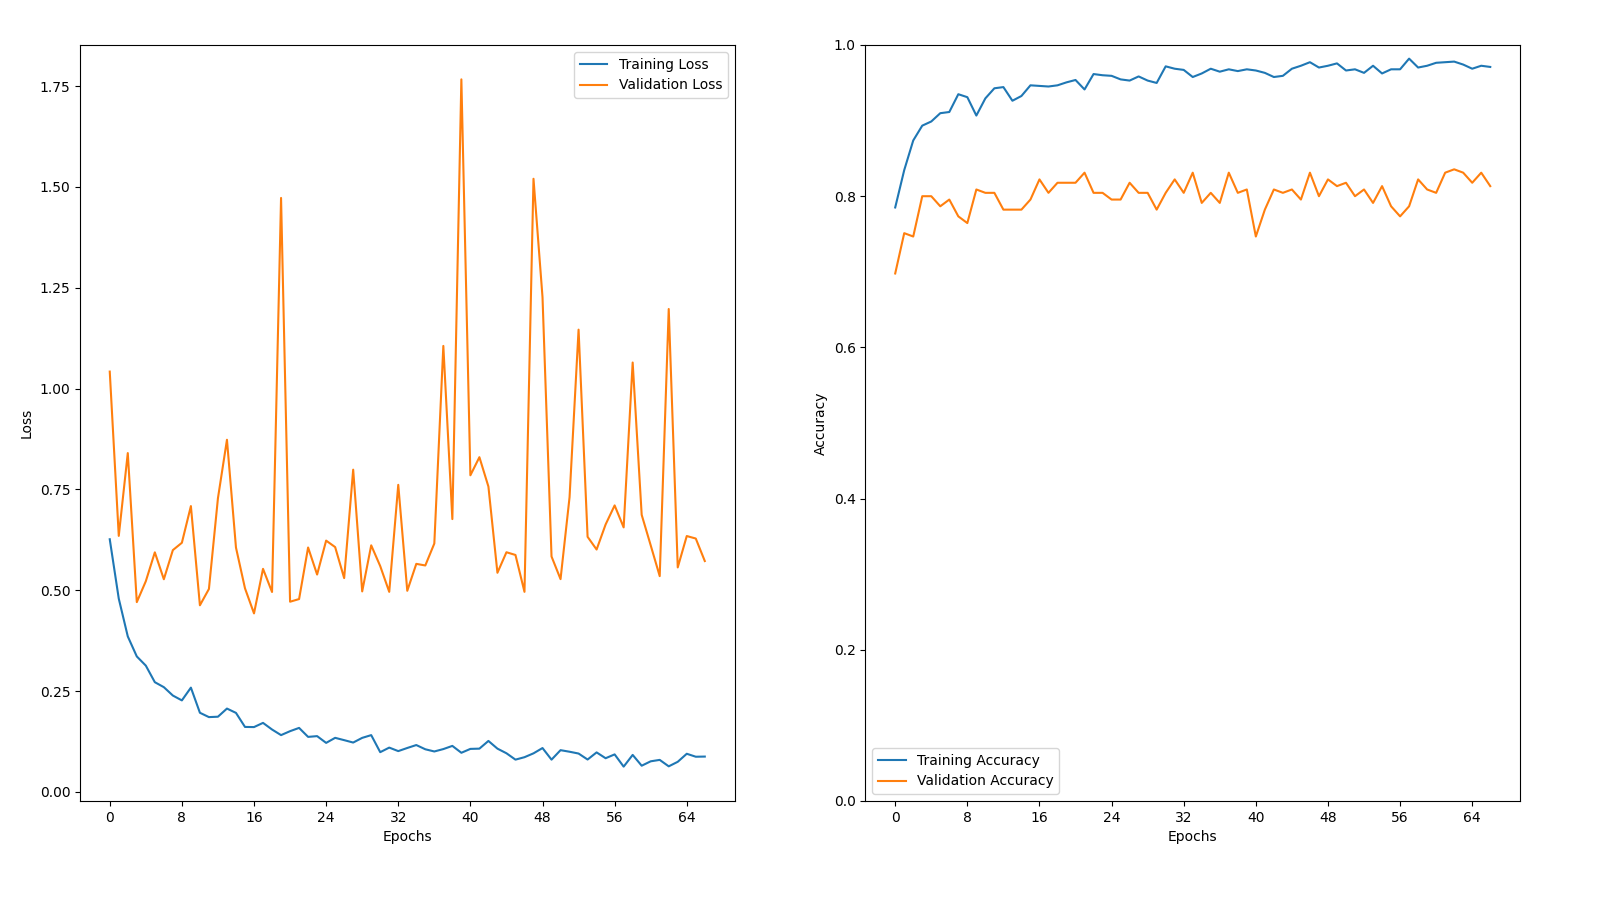
\includegraphics[width=0.75\textwidth]{loss_and_accuracy_task_3.png}
    \caption{Training and validation losses and accuracies of the fine-tuned model.}
    \label{fig:task3_loss_accuracy}
\end{figure}

As expected, the model converges very quickly, since AlexNet is already a very good model for image classification,
and through the use of transfer learning it only has to adapt to the new training set.

\pagebreak

The confusion matrix of the model on the test set is as follows:
\begin{figure}[h]
    \centering
    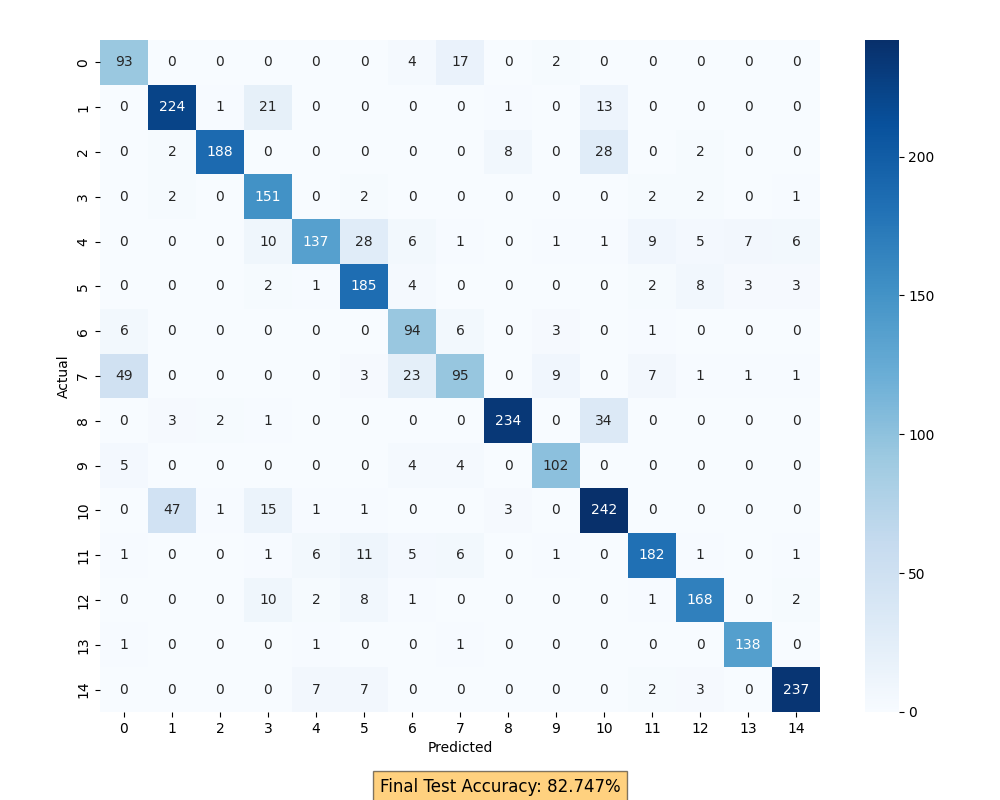
\includegraphics[width=0.66\textwidth]{confusion_matrix_task_3.png}
    \caption{Confusion matrix of the fine-tuned model on the test set.}
    \label{fig:task3_confusion_matrix}
\end{figure}

The final average test accuracy of the fine-tuned model is 83.3±0.6\%.

\subsection{SVM classifier}
Another possible approach for transfer learning is to use the feature extractor part of AlexNet 
as a feature extractor for a One-vs-One SVM classifier\footnote{The SVM classifier is linear and uses a C value of 1.0. Using a non-linear SVM classifier or a different C value didn't improve the performance of the model.}:
\begin{lstlisting}[language=Python]
from sklearn import svm

features_layer = models.alexnet(weights=AlexNet_Weights.DEFAULT).features
for param in self.features_layer.parameters():
    param.requires_grad = False
svm = svm.SVC(kernel="linear", C=1.0)
\end{lstlisting}
A function to fit the SVM classifier is then defined:
\begin{lstlisting}[language=Python]
def fit_svm(dataloader, epochs):
    features = []
    labels = []
    for _ in range(epochs):
        for x, y in iter(dataloader):
            features.append(np_features(x))
            labels.append(y.detach().numpy())
    features = np.concatenate(features)
    labels = np.concatenate(labels)
    svm.fit(features, labels)
\end{lstlisting}
\pagebreak
\begin{lstlisting}[language=Python]
def np_features(x):
    features = features_layer(x)
    features = features.view(x.size(0), -1)
    return features.detach().numpy()
\end{lstlisting}

By one-hot encoding the prediction, the SVM classifier can be fit to the training data and be used as a classifier for the test data as follows:
\begin{lstlisting}[language=Python]
def forward(x):
    features = features_layer(x)
    features = features.view(x.size(0), -1)
    features_np = features.detach().numpy()
    predictions = svm.predict(features_np)
    probabilities = np.zeros((predictions.shape[0], svm.classes_.shape[0]))
    probabilities[np.arange(predictions.shape[0]), predictions] = 1
    return torch.from_numpy(probabilities)
\end{lstlisting}
The confusion matrix of the model on the test set is as follows:
\begin{figure}[h]
    \centering
    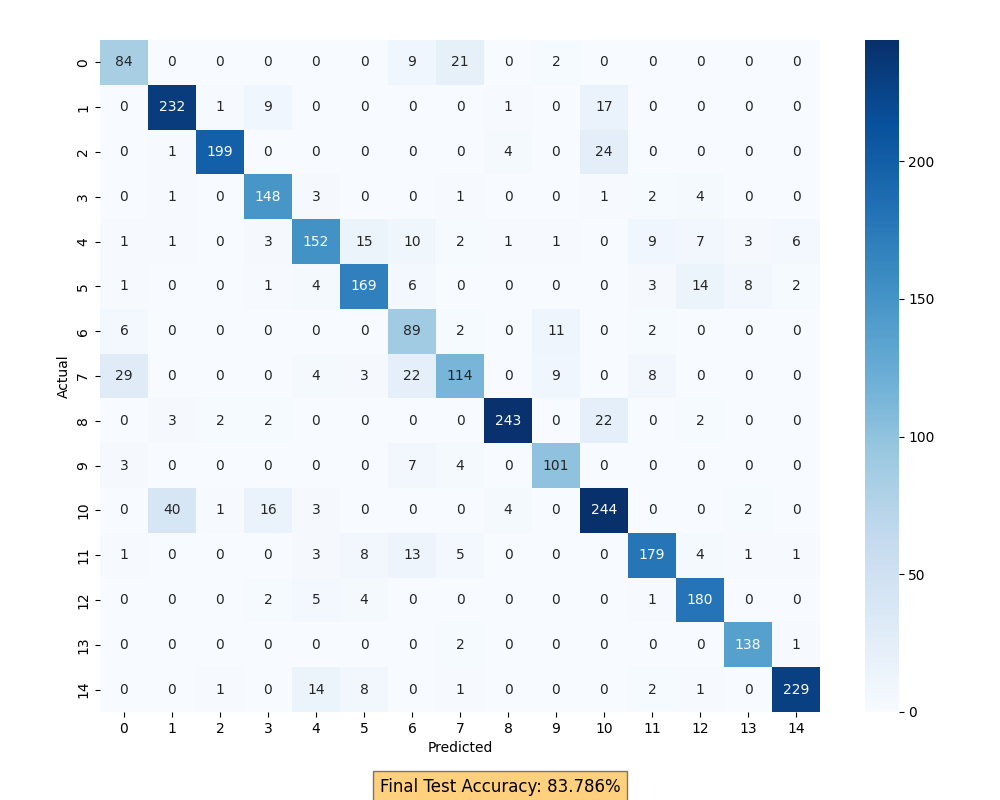
\includegraphics[width=0.66\textwidth]{confusion_matrix_task_3_svm.png}
    \caption{Confusion matrix of the SVM classifier on the test set.}
    \label{fig:task3_confusion_matrix_svm}
\end{figure}

The final average test accuracy of the SVM classifier is 84.4±0.5\%.

\begin{table}[h]
    \begin{tabular}{|l|l|l|}
        \hline
        \textbf{Model} & \textbf{Avg test accuracy} & \textbf{Confidence interval}\tablefootnote{95\% confidence interval over 10 runs using the t-distribution.} \\
        \hline
        Base reference model & 27.9\% & 1.9\% \\
        Base model + data augmentation & 43.7\% & 2.5\% \\
        Base model + data augmentation + regularization & 54.2\% & 1.9\% \\
        Ensemble model & 62.7\% & N/A \\
        Fine-tuned AlexNet & 83.3\% & 0.6\% \\
        AlexNet feature extractor + OvO SVM & 84.4\% & 0.5\% \\
        \hline
    \end{tabular}
    \caption{Comparison of the results of the different models.}
    \label{tab:comparison_table}
\end{table}

\pagebreak

\bibliographystyle{apalike}
\bibliography{references}
\addcontentsline{toc}{section}{References}
\end{document}